\documentclass{article}
\usepackage[utf8]{inputenc}
\usepackage[margin = 0.8in]{geometry}
\usepackage{graphicx}
\usepackage{amsmath, amssymb}
\usepackage{subcaption}
\usepackage{multirow}
\usepackage{mathtools}
\usepackage{float}
\usepackage{pythonhighlight}


\title{RBE595 - Homework 1}
\author{Keith Chester}
\date{Due date: January 15, 2024}

\begin{document}
\maketitle

\section*{Task 1}

We are tasked with analyzing the sensor presented in this problem, aiming to classify the usefulness of the sensor with our given reliability.

First, the provided information - the sensor is depicted as a poor black and white camera capable of detecting if a door is open with a success rate of 60\%, and senses the door being closed 80\% of the time correctly. Thus our probabilities are:

\begin{equation}
    \begin{split}
        p(z_t = 1 \mid x_t - 1) = 0.6 \\
        p(z_t = 0 \mid x_t - 1) = 0.4 \\
        p(z_t = 1 \mid x_t = 0) = 0.2 \\
        p(z_t = 0 \mid x_t = 0) = 0.8
    \end{split}
\end{equation}

We also know that robot manipulator is similarly imperfect. If the door is closed and the robot attempts to open it, it will succeed 80\% of the time. If no action is taken, the state will remain unchanged (obviously). We can thus express the following about our manipulator:

\begin{equation}
    \begin{split}
        p(X_t = \textbf{is\_open} \mid U_t = \textbf{push}, X_{t_1} = \textbf{is\_open}) = 1.0 \\
        p(X_t = \textbf{is\_closed} \mid U_t = \textbf{push}, X_{t_1} = \textbf{is\_open}) = 0.0 \\
        p(X_t = \textbf{is\_open} \mid U_t = \textbf{push}, X_{t_1} = \textbf{is\_closed}) = 0.8 \\
        p(X_t = \textbf{is\_closed} \mid U_t = \textbf{push}, X_{t_1} = \textbf{is\_closed}) = 0.2 \\
        \\
        p(X_t = \textbf{is\_open} \mid U_t = \textbf{noop}, X_{t_1} = \textbf{is\_open}) = 1.0 \\
        p(X_t = \textbf{is\_closed} \mid U_t = \textbf{noop}, X_{t_1} = \textbf{is\_open}) = 0.0 \\
        p(X_t = \textbf{is\_open} \mid U_t = \textbf{noop}, X_{t_1} = \textbf{is\_closed}) = 0.0 \\
        p(X_t = \textbf{is\_closed} \mid U_t = \textbf{noop}, X_{t_1} = \textbf{is\_closed}) = 1.0
    \end{split}
\end{equation}

...wherein \textbf{noop} is a no operation, or \textbf{doing nothing}.

If we were to start at $t=1$, taking no action but measuring an open door, we would have the following belief:

\begin{equation}
    \begin{split}
        \overline{bel}(x_1) \int p(x_1 \mid u_1, x_0) bel(x_0)dx_0 \\
        = \sum_{x_0} p(x_1 \mid u_1, x_0) bel(x_0) \\
        = p(X_1 \mid U_1 = \textbf{noop}, x_0 = \textbf{is\_open}) bel(x_0 = \textbf{is\_open}) + \\
        p(X_1 \mid U_1 = \textbf{noop}, x_0 = \textbf{is\_closed}) bel(x_0 = \textbf{is\_closed}) \\
    \end{split}
\end{equation}

We have two possible states for $X_1$ - the door can have either \textbf{is\_open} or \textbf{is\_closed}. Expanding this for each possible state:

\begin{equation}
    \begin{split}
        \overline{bel}(X_1=\textbf{is\_open}) = \\
        p(X_1 = \textbf{is\_open} \mid U_1 = \textbf{noop}, X_0 = \textbf{is\_open}) bel(X_0 = \textbf{is\_open}) + \\
        p(X_1 = \textbf{is\_open} \mid U_1 = \textbf{noop}, X_0 = \textbf{is\_closed}) bel(X_0 = \textbf{is\_closed}) = \\
        1.0 * 0.5 + 0.0 * 0.5 = 0.5 \\
    \end{split}
\end{equation}

\begin{equation}
    \begin{split}
        \overline{bel}(X_1=\textbf{is\_closed}) = \\
        p(X_1 = \textbf{is\_closed} \mid U_1 = \textbf{noop}, X_0 = \textbf{is\_open}) bel(X_0 = \textbf{is\_open}) + \\
        p(X_1 = \textbf{is\_closed} \mid U_1 = \textbf{noop}, X_0 = \textbf{is\_closed}) bel(X_0 = \textbf{is\_closed}) = \\
        0.0 * 0.5 + 1.0 * 0.5 = 0.5 \\
    \end{split}
\end{equation}

This makes sense - our \textbf{noop} is literally doing nothing, and thus has no effect on the state of the door. We have to consider our measurement, however, which, as we covered earlier, is noisy. Thus:

\begin{equation}
    bel(x_1) = \eta p(z_1 \mid x_1) \overline{bel}(x_1)
\end{equation}

\begin{equation}
    \begin{split}
        bel(X_1 = \textbf{is\_open}) = \\
        \eta p(Z_1 = \textbf{door\_open} \mid X_1 = \textbf{is\_open}) \overline{bel}(X_1 = \textbf{is\_open}) = \\
        \eta 0.6 * 0.5 = \eta 0.3
    \end{split}
\end{equation}

\begin{equation}
    \begin{split}
        bel(X_1 = \textbf{is\_closed}) = \\
        \eta p(Z_1 = \textbf{door\_open} \mid X_1 = \textbf{is\_closed}) \overline{bel}(X_1 = \textbf{is\_closed}) = \\
        \eta 0.2 * 0.5 = \eta 0.1
    \end{split}
\end{equation}

We can now calculate $\eta$:

\begin{equation}
    \begin{split}
        \eta = \frac{1}{0.3 + 0.1} = \frac{1}{0.4} = 2.5
    \end{split}
\end{equation}

Which means:

\begin{equation}
    \begin{split}
        bel(X_1 = \textbf{is\_open}) = 2.5 * 0.3 = 0.75 \\
        bel(X_1 = \textbf{is\_closed}) = 2.5 * 0.1 = 0.25
    \end{split}
\end{equation}

We iterate on this for the next timestep, leading us to\dots

\begin{equation}
    \begin{split}
        \overline{bel}(X_2=\textbf{is\_open}) = 1 * 0.75 + 0.8 * 0.25 = 0.95 \\
        \overline{bel}(X_2=\textbf{is\_closed}) = 0 * 0.75 + 0.2 * 0.25 = 0.05 \\
    \end{split}
\end{equation}

\begin{equation}
    \begin{split}
        bel(X_2 = \textbf{is\_open}) = \eta 0.6 * 0.95 = 0.983 \\
        bel(X_2 = \textbf{is\_closed}) = \eta 0.2 * 0.05 = 0.017
    \end{split}
\end{equation}

Thus, while we have a set probability of success for our sensor, we must also consider the success probability of our actuator and prior actions.

\section*{Task 2}

In this problem we were tasked to implement a Bayes filter from scratch in a language of our choice. For simplicity, Python was chosen. The attached files, \textbf{task2.py}, contains the salient code for this task. A generic Bayes Filter class is created and reused for the given tasks.

The class in question:

\begin{python}
    class BayesFilter:
    """
    This is a generic implementation of a Bayes Filter, with no
    application-specific implementation details. It simply is
    initiated with a set of prior measurements and initial belief
    of probability. Then you may predict / update as steps to
    iteratively improve the belief of whatever you're trying to
    estimate.
    """

    def __init__(
    self,
    initial_belief: float,
    state_mapping: Dict[int, Dict[int, Dict[int, float]]],
    sensor_probabilities: Dict[int, Dict[int, float]],
    ):
    self.state_mapping = state_mapping
    self.sensor_probabilities = sensor_probabilities
    self.belief = initial_belief
    self.__belief_history: List[float] = [initial_belief]

    def prediction(self, action: int):
    """
    prediction step of the Bayes Filter, returning a new belief
    based on the action taken.
    """
    positive = self.state_mapping[OPEN][action][OPEN] * self.belief
    negative = self.state_mapping[CLOSED][action][OPEN] * (1 - self.belief)
    belief = positive + negative

    return belief

    def update(self, measurement: int):
    """
    update the belief based on the measurement
    """
    is_open = self.sensor_probabilities[measurement][OPEN] * self.belief
    is_closed = self.sensor_probabilities[measurement][CLOSED] * (1 - self.belief)

    normalized_belief = is_open / (is_open + is_closed)

    return normalized_belief

    def calculate_belief(self, action: float, measurement: float) -> float:
    """
    calculate_belief generates a new belief based on the action
    and measurement, calling the prediction and update steps of
    the Bayes filter accordingly.
    """
    self.belief = self.prediction(action)
    self.belief = self.update(measurement)
    self.__belief_history.append(self.belief)
    return self.belief

    def plot_history(self):
    """
    plot_history plots the belief history of the Bayes filter
    """
    plt.plot(self.__belief_history)
    plt.ylabel("State Belief")
    plt.xlabel("Steps")
    plt.title("Bayes Filter Belief History")
    return plt
\end{python}

...the class provides an instantiation with an initial belief, and calculates the belief by referencing both the prediction and measurement update steps. It also tracks overall history of beliefs and plots it on request.

The \textbf{task2.py} file will execute each task in order. We share their outputs here for easier reference.

\subsection*{Question 1}

\textbf{If the robot always takes the action “do nothing” and always receives the measurement “door open” how many iterations will it take before the robot is at least 99.99\% certain the door is open?"}

\begin{python}
    initial_belief = 0.5
    filter = BayesFilter(initial_belief, state_mapping, sensor_probabilities)
    action = NOOP
    measurement = OPEN

    iterations = 0
    while filter.belief < 0.9999:
    iterations += 1
    filter.belief = filter.calculate_belief(action, measurement)
    print(f"Reached {filter.belief} in {iterations} iterations.")
\end{python}

Our program outputted that the target belief of 99.99\% was reached within \textbf{9} iterations.


\begin{figure}[H]
    \centering
    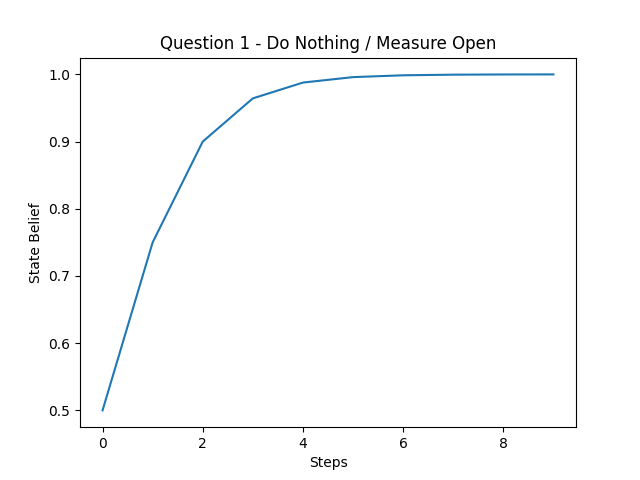
\includegraphics[width = 0.45\textwidth]{q1.png}
\end{figure}

\subsection*{Question 2}
\textbf{If the robot always takes the action “push” and always receives the measurement “door open” how many iterations will it take before the robot is at least 99.99\% certain the door is open?"}


Our program reached reached 99.9989\% in \textbf{4} iterations.

\begin{figure}[H]
    \centering
    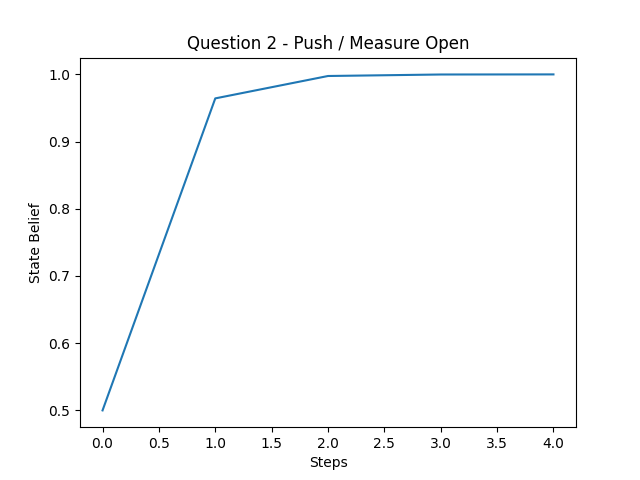
\includegraphics[width = 0.45\textwidth]{q2.png}
\end{figure}

\subsection*{Question 3}
\textbf{If the robot always takes the action “push” and always receives the measurement “door closed” what is the steady state belief about the door? Include both the state and the certainty.}

In this question we are iterating on the belief until the resulting delta between a given belief $b(x_t)$ and $b(x_{t-1})$ is smaller or equal to than $0.0001$.

\begin{python}
    initial_belief = 0.5
    filter = BayesFilter(initial_belief, state_mapping, sensor_probabilities)
    action = PUSH
    measurement = CLOSED

    minimum_delta = 0.0001
    iterations = 0
    delta = 100.0  # Just a large number to start

    while delta > minimum_delta:
    iterations += 1
    old_belief = filter.belief
    filter.calculate_belief(action, measurement)
    delta = abs(old_belief - filter.belief)

    print(f"Our delta is too small ({delta}), so we are calling it steady now.")
    print(f"Completed in {iterations} iterations.")
    print(f"Final belief: {filter.belief}")
\end{python}

Our loop was terminated in \textbf{10} iterations, where it held a \textbf{99.99\%} belief.

\begin{figure}[H]
    \centering
    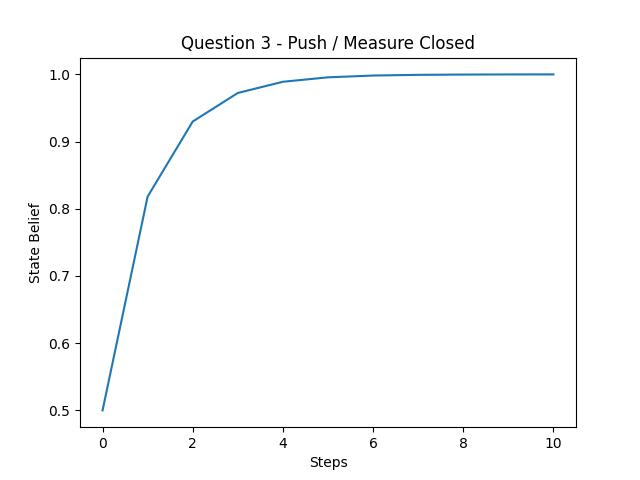
\includegraphics[width = 0.45\textwidth]{q3.png}
\end{figure}


\end{document}